%%%%%%%%%%%%%%%%%%%%%%%%%%%%%%%%%%
% EEE Report Template
% University of Southampton
%
% authors: George Brown (gb4g15)
%          Rhys Thomas  (rt8g15)
%
% edited : 2016/02/05
%%%%%%%%%%%%%%%%%%%%%%%%%%%%%%%%%%

\documentclass[a4paper]{article}

%%%%%%%%%%%%%%%%%%%%%%%%%%%%%%%%%%
% PACKAGES
%%%%%%%%%%%%%%%%%%%%%%%%%%%%%%%%%%
\usepackage{multicol} % multiple columns
\usepackage{fancyhdr} % page number in bottom right
\usepackage{graphicx} % images
\usepackage{float} % float image in columns, gives [H]
\usepackage{amsmath, amssymb} % maths symbols / environments
\usepackage{times} % times font instead of computer modern
\usepackage{IEEEtrantools} % et al referencing
\usepackage{booktabs} % nice replacements for \hline in tables
\usepackage{calc} % calculating textwidth-2cm etc.
\usepackage[none]{hyphenat} % no hyphenation
\usepackage{geometry} % Page Margins
\usepackage{hyperref} % PDF metadata setup.
\usepackage{mathptmx} % Use times font face for maths
\usepackage{caption} % Tighter caption control.

\usepackage{lipsum} % Temporary to generate body text

%%%%%%%%%%%%%%%%%%%%%%%%%%%%%%%%%%
% TITLE AND AUTHOR
%%%%%%%%%%%%%%%%%%%%%%%%%%%%%%%%%%
% This info is reused, set it here and it'll be updated globally.
\newcommand{\docTitle}{Lab Report Template}
\newcommand{\docAuthor}{George Brown, Rhys Thomas}

% Put the metadata in the PDF output.
\hypersetup{
    unicode=true,
    pdftitle={\docTitle{}},
    pdfauthor={\docAuthor{}}
}

%%%%%%%%%%%%%%%%%%%%%%%%%%%%%%%%%%
% FORMATTING REQUIREMENTS
%%%%%%%%%%%%%%%%%%%%%%%%%%%%%%%%%%
\geometry{a4paper, top=2.5cm, bottom=2.5cm, left=2cm, right=2cm}
\linespread{1.05} % 1.05x line spacing.
\setlength{\columnsep}{0.7cm} % 0.7cm column spacing.
\setlength{\multicolsep}{0cm}
\setlength{\parskip}{6pt} % 6pt skip between paragraphs
\setlength{\parindent}{0pt}
\newcommand{\figsquish}{\vspace{-5mm}} % Hack to fix poor [H] figure spacing

% Captions
% Table captions go above, 6pt space, small (9pt) roman font,
% roman numeral counting.
\captionsetup[table]{position=above, skip=6pt, font={small, rm}}
\renewcommand\thetable{\Roman{table}}
% Figure captions go below, 5pt space, small (9pt) roman font.
\captionsetup[figure]{position=below, skip=5pt, font={small, rm}}

%%%%%%%%%%%%%%%%%%%%%%%%%%%%%%%%%%
% SECTION REQUIREMENTS
%%%%%%%%%%%%%%%%%%%%%%%%%%%%%%%%%%
\usepackage{titlesec}
\titlelabel{\thetitle.\hspace{0.5cm}} % Dot after number for sections
% Format is 10pt, so \large = 12pt, \normalsize=10pt
\titleformat*{\section}{\large\bfseries}
\titlespacing*{\section}{0cm}{4pt}{4pt} % 6pt from \parindent
\titleformat*{\subsection}{\normalsize\bfseries}
\titlespacing*{\subsection}{0cm}{0pt}{0pt} % 6pt from \parindent

% Set up footer.
\pagestyle{fancy}
\fancyhf{}
\renewcommand{\headrulewidth}{0pt}
\rfoot{\thepage} % page number, bottom right of page

%%%%%%%%%%%%%%%%%%%%%%%%%%%%%%%%%%
% DOCUMENT BEGIN
%%%%%%%%%%%%%%%%%%%%%%%%%%%%%%%%%%

\begin{document}

% Pull in the IEEE referencing setup stuff.
\bstctlcite{IEEEexample:BSTcontrol}

%%%%%%%%%%%%%%%%%%%%%%%%%%%%%%%%%%
% HEADER
%%%%%%%%%%%%%%%%%%%%%%%%%%%%%%%%%%
{
    \centering
    % Use size 28 font. 1.05x gives 29.4pt line spacing.
    \fontsize{28pt}{29.4pt} \selectfont
    \docTitle\\
    \vspace{25pt}
    % Name block.
    \fontsize{11pt}{11.55pt}\selectfont
    \docAuthor\\
    \fontsize{10pt}{10.5pt}\selectfont
    \textit{gb4g15@soton.ac.uk, rt8g15@soton.ac.uk} \\ % You Email
    \textit{Personal Tutor: Dr Stuart Boden, Dr Jeff Reeve} \\ % Your tutor
}
\vspace{25pt}

%%%%%%%%%%%%%%%%%%%%%%%%%%%%%%%%%%
% ABSTRACT
%%%%%%%%%%%%%%%%%%%%%%%%%%%%%%%%%%
{
% No additional column spacing since we've set it strictly.
\setlength{\tabcolsep}{0cm}
\centering
\begin{tabular}{p{2cm}p{\textwidth-2cm}}
    
    Abstract: &
    
    This is the body of my abstract. It will tell you all about how excellent 
    my paper is! Please give me lots of money, since as is detailed herein, I 
    have a truly excellent patent opportunity. In reality, this is a template 
    for ECS lab reports, written in \LaTeX. IEEE style references are 
    generated using \textsc{Bib}\TeX and IEEEtran.
\end{tabular}  
}
\vspace{25pt}

%%%%%%%%%%%%%%%%%%%%%%%%%%%%%%%%%%
% BODY
%%%%%%%%%%%%%%%%%%%%%%%%%%%%%%%%%%
\begin{multicols*}{2}

\section{Introduction}

This text demonstrates how you might go about referencing items in the text. 
For example, you can find a table of my favourite elements in 
Table~\ref{tab:fav-elements}. There is also Figure~\ref{fig:hdd-crash}, which 
shows one of the many situations that can occur where you'll really wish you'd 
made a backup. Equation~\ref{eq:einstein} will teach you all about the true 
nature of matter, while Figure~\ref{fig:pid-loop} will conjure terrible 
memories of D1.

\section{Formatting Example}

You may wish to change your font at some point in your document to provide, 
for example: \textbf{bold text}, \textit{italic text}, or \emph{environment 
sensitive \emph{emphasized} text}. You might also like to include some code, 
like this: \texttt{printf("LAH-tekh not lay-teks");}.

In some cases, you might also like to have maths inline, say to provide a 
variable like $\phi_0$, or to include an expression like $3+4=7$.

This document has been setup to automatically generate IEEE references and 
citations. Most good online journals provide a \textsc{Bib}\TeX reference, 
which makes life very easy, simply copy the contents of the provided 
\texttt{.bib} file, and then make a reference with \verb|\cite{ref}|. The 
result is something like \cite{ref1}.

The remainder of the text in this document is total rubbish, so don't bother 
trying to read it! The source however will still be useful!

\section{Lorem}
\lipsum[1]

\begin{figure}[H]
    \centering
    \includegraphics[width=\columnwidth]{pid}
    \caption{A nice vector figure.}
    \label{fig:pid-loop}
\end{figure}
\figsquish

\subsection{Ipsum}
\paragraph{Dolor}
\lipsum[2-3]

\begin{figure}[H]
    \centering
    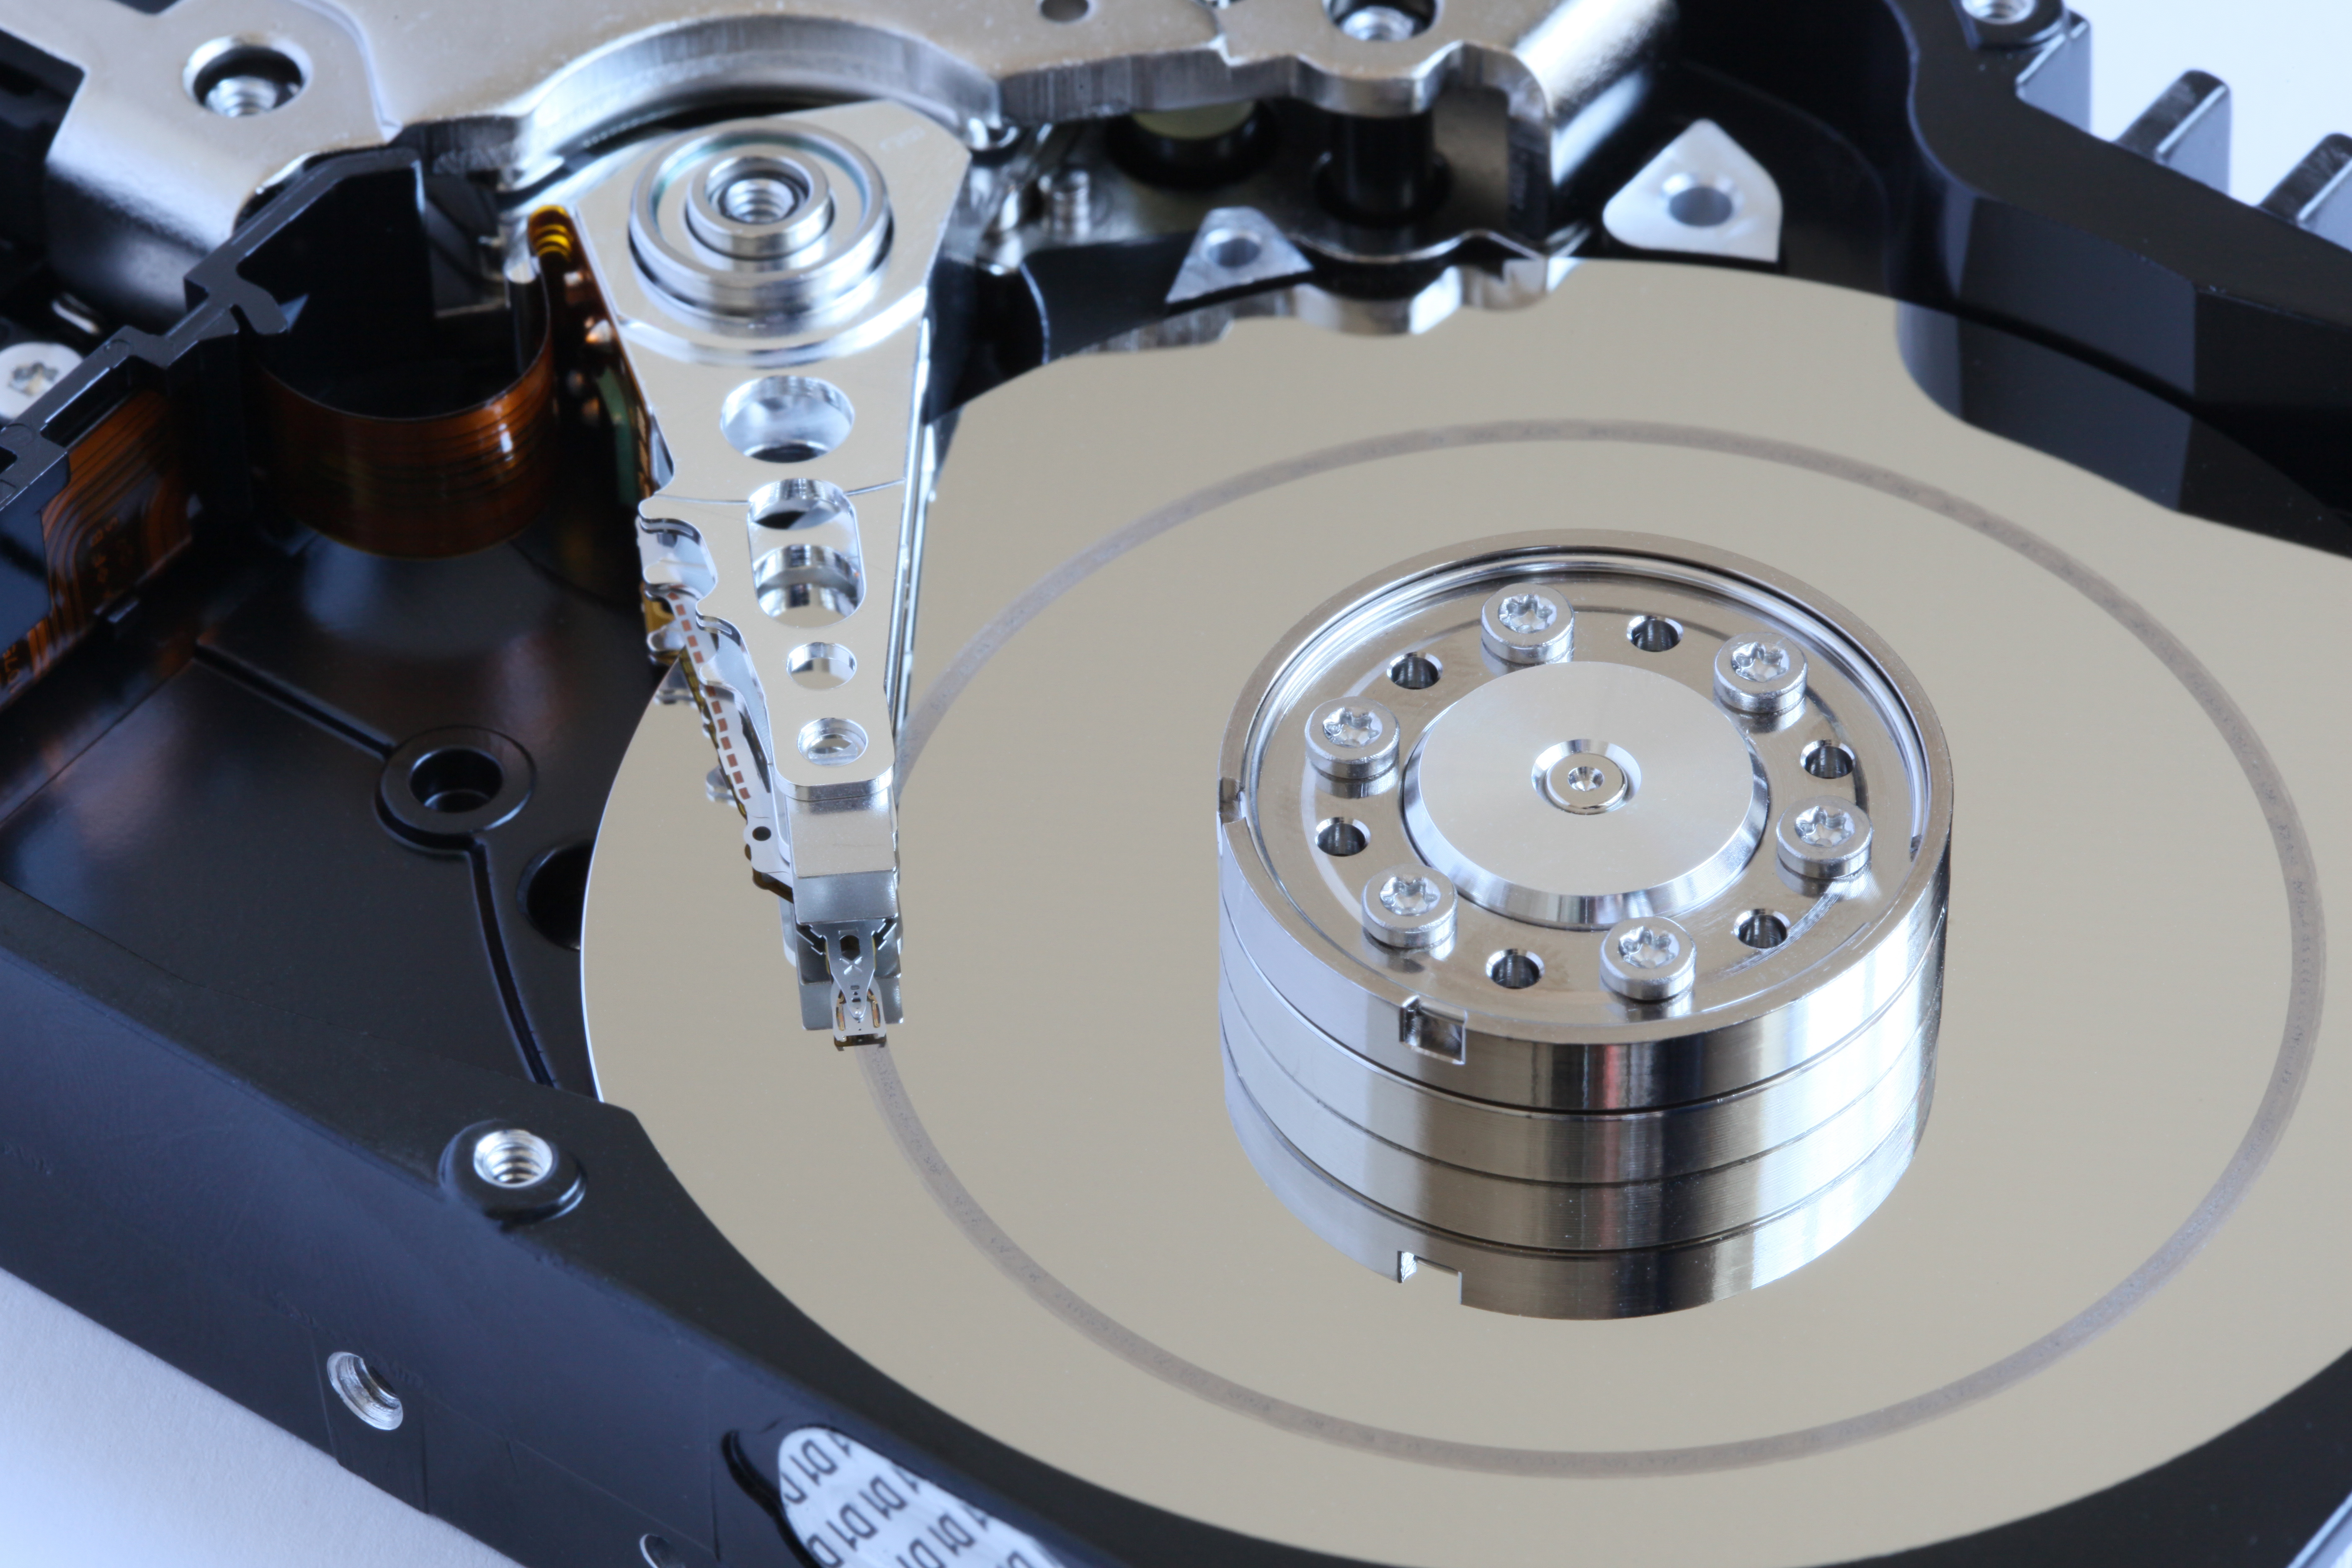
\includegraphics[width=\columnwidth]{hdd-crash}
    \caption{I hope you make regular backups\ldots}
    \label{fig:hdd-crash}
\end{figure}
\figsquish

\lipsum[4-7]

\begin{table}[H]
    \centering
    \caption{My Favourite Elements}
    \begin{tabular}{ccc}
        Symbol & Name & Atomic Number \\
        \midrule
        H & Hydrogen & 1 \\
        Sn & Tin &  50\\
        W & Tungsten & 74
    \end{tabular}
    \label{tab:fav-elements}
\end{table}
\figsquish
\lipsum[14-16]

\figsquish
\begin{gather}
    E = MC^2 \label{eq:einstein} \\
    Q = \frac{f_0^\prime}{f_2 - f_1} = \frac{f_0^\prime}{bandwidth} =
    \frac{1}{2\pi f_0^\prime CR} =
    \frac{2\pi f_0^\prime L}{R} \label{eq:quality}\\
    f_0 = \frac{1}{2\pi\sqrt{LC}}
\end{gather}
\lipsum[17-20]

Figure~\ref{fig:hdd-crash} by Alchemist-hp at wikimedia.org.
Figure~\ref{fig:pid-loop} by TravTigerEE at wikimedia.org.

%%%%%%%%%%%%%%%%%%%%%%%%%%%%%%%%%%
% BIBLIOGRAPHY
%%%%%%%%%%%%%%%%%%%%%%%%%%%%%%%%%%
\nocite{*} % show all references even without citation
% to cite use "bla bla"~\cite{ref_label} -> "bla bla" [1]
\bibliographystyle{IEEEtran}
% IEEEabrv abbreviates journal titles in accordance to IEEE standards 
\bibliography{IEEEabrv,mybib}

\end{multicols*}
\end{document}

